\section{Sec.~VIII: Emergence of bulk geometric concepts}

Sec.~VII established that a bulk region \emph{is} a boundary algebra. This section pushes that identification
to its limit: causal structure, the formation of a horizon, and even whether two boundary theories are joined
by a wormhole at all, can each be read directly off the type and commutant structure of boundary algebras —
with no bulk metric assumed anywhere in the argument. This closes the two puzzles flagged back in Sec.~VI.C
(the factorization puzzle was already resolved there; the meeting-behind-the-horizon puzzle is resolved here,
in Sec.~VIII.B).

\subsection{Sec.~VIII.A: algebraic characterization of bulk causal structure}

\subsubsection*{Why boundary commutants can encode more than boundary causality}

Boundary operators separated in a spacelike way automatically commute — ordinary microcausality. But
\emph{timelike}-separated boundary operators are not required to commute at all; whether they do depends on
the specific representation, which is fixed by the state's two-point functions. This freedom is not a bug —
it's exactly the room needed for boundary commutant structure to encode something richer than boundary
causality alone: by subregion-subalgebra duality, it encodes bulk causal structure, in one higher dimension.

\subsubsection*{The causal depth parameter}

Recall from Sec.~VI.B (eq.~6.33) that in empty AdS, a boundary time band $I_w$ generates the entire algebra,
$Y_{I_w}=B(\HH_\Omega^{\text{GNS}})$, once $w\ge\pi R$ — geometrically, $\pi R$ is exactly the minimal width
for which light rays from the band already cover an entire bulk Cauchy slice. This motivates a purely
boundary-intrinsic definition:

\begin{quote}
\textbf{Definition (causal depth $T(t)$).} For a single-sided semiclassical state $\ket\Psi$, $T(t)$ is the
largest $w$ for which the time-band algebra $Y_{I_w(t)}$ (centered at boundary time $t$) still has a
\emph{nontrivial} commutant.
\end{quote}

For empty AdS, $T(t)=\pi R$: finite and time-independent, matching the geometric statement that light rays
from a band of exactly that width already reach everywhere. For a general horizon-free asymptotically-AdS
geometry, $T(t)$ is expected to stay finite for all time. For a single-sided eternal black hole (Fig.~26(b) of
the paper), by contrast, $Y_{I_w}$ has a \emph{nontrivial} commutant for \emph{every} finite $w$ — no matter
how wide a time band you take, you can never quite reach the full exterior algebra (only in the strict
$w\to\infty$ limit does the commutant become trivial) — so $T(t)=\infty$, for all $t$: \textbf{a purely
boundary-intrinsic signature of a horizon, requiring no bulk metric to state.} For a black hole formed by
collapse (Fig.~25 again), $T(t)$ starts finite and grows monotonically, diverging only as $t\to\infty$ — the
boundary-side signature of a horizon actually \emph{forming}, in real time, rather than always having been
there.

A two-sided version, $T_R(t)$, is defined the same way but using the \emph{relative} commutant of $Y_{I_w}$
within $Y_R$ (the right boundary's own single-trace algebra) — for the thermofield double below
$T_{\text{HP}}$, this reduces to ordinary empty AdS's $\pi R$; above $T_{\text{HP}}$, it diverges for all
time, exactly reproducing eq.~7.40's bifurcating-horizon diagnostic from Sec.~VII.E in this new language.

\begin{figure}[htbp]
\centering
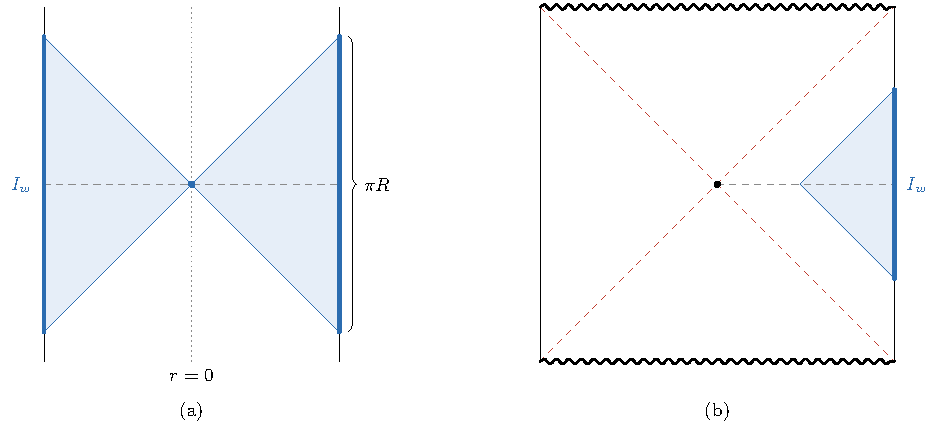
\includegraphics[width=0.90\textwidth]{figs/fig_causal_depth.pdf}
\caption{The causal depth parameter $T(t)$ as an algebraic detector of horizons. (a) In empty AdS, a boundary time band $I_w$ of width $w \ge \pi R$ sends light rays that meet at the bulk center $r=0$ and cover an entire Cauchy slice, driving the commutant to triviality ($Y_{I_w}' = \mathbb{C}\mathbf{1}$) and giving a finite causal depth $T = \pi R$. (b) In a black hole spacetime, boundary light rays asymptotically wrap around the horizon without crossing, so $Y_{I_w}' \ne \mathbb{C}\mathbf{1}$ for all finite $w$. The causal depth diverges: $T = \infty$, serving as a purely algebraic boundary diagnostic of a horizon.}
\label{fig:causal_depth}
\end{figure}

\subsubsection*{$T$ as a measure of lost determinism}

Here's a genuinely illuminating reframing of what $T$ is measuring, worth holding onto because it explains why
this whole construction is possible at all. At finite $N$, knowing the operator algebra on a single Cauchy
slice determines the whole theory (ordinary causal time evolution, the time-slice axiom of Sec.~IV.D.3). In
the strict large-$N$ limit, this stops being true — there are no equations of motion relating single-trace
operators at different times (Sec.~VI.A) — but the theory isn't completely disconnected across time either:
correlations (encoded in two-point functions) still relate a time band's algebra to the rest of the theory,
just not through equations of motion. $T$ is exactly the minimal width of a band whose algebra is
\emph{still enough}, via these correlations rather than dynamics, to recover the whole system. Read this way,
\textbf{$T=0$ is full determinism (an honest equation of motion); $T$ finite is a partial, quantifiable loss of
determinism; $T=\infty$, as in a black hole, is a complete loss of determinism — no finite window of boundary
time, however wide, is ever enough.} The emergence of the bulk radial direction is, in this precise sense,
tied to the boundary theory progressively losing determinism as $N\to\infty$.

(The paper makes this fully rigorous by relating $T$ to a classical object from harmonic analysis called the
\emph{exponential type} of the spectral function $\rho(\omega)$ — the Fourier transform of the commutator
$\braket{\Psi|[O(t),O(t')]|\Psi}$ (eqs.~8.1--8.5) — connecting it to an old question of Kolmogorov's about how
long you must observe a chaotic classical system before you can predict its entire future. This machinery is
flagged here for completeness; the physical content that matters going forward is the definition of $T$ itself
and what it measures, not the harmonic-analysis technique used to compute it in specific examples.)

\subsubsection*{Worked calculation: spectral functions and the divergence of causal depth}

To make the causal depth parameter $T(t)$ mathematically transparent, let us compute the spectral function $\rho(\omega)$ explicitly in two contrasting backgrounds: empty AdS versus a thermal black hole.
The spectral function is defined as the Fourier transform of the boundary commutator:
\[
\rho(\omega) \equiv \int_{-\infty}^\infty dt\, e^{i\omega t}\, \braket{\Psi|\big[O(t),\, O(0)\big]|\Psi}
\]
\begin{enumerate}
\item \textbf{Vacuum state $\ket\Omega$ (Empty AdS)}:
In global $\text{AdS}_{d+1}$ of radius $R$, the boundary CFT spectrum consists of discrete primaries and descendants with energies $\omega_n = (\Delta + 2n)/R$ for $n \in \mathbb{N}_0$. The Wightman function is:
\[
\braket{\Omega|O(t)O(0)|\Omega} = \sum_{n=0}^\infty c_n e^{-i(\Delta + 2n)t/R}
\]
The commutator is therefore:
\[
\braket{\Omega|\big[O(t),O(0)\big]|\Omega} = -2i \sum_{n=0}^\infty c_n \sin\big((\Delta + 2n)t/R\big)
\]
Its Fourier transform $\rho(\omega)$ is a discrete sum of delta functions:
\[
\rho(\omega) = 2\pi \sum_{n=0}^\infty c_n \Big(\delta\big(\omega - (\Delta+2n)/R\big) - \delta\big(\omega + (\Delta+2n)/R\big)\Big)
\]
Notice that $\rho(\omega) = 0$ identically in the frequency bandgap $|\omega| < \Delta/R$. By the classical Paley--Wiener theorem of Fourier analysis, a spectral function with this discrete bandgap structure has a finite exponential type:
\[
T = \pi R < \infty
\]
Thus a boundary time band of finite width $w \ge \pi R$ is sufficient to reconstruct all operators in the vacuum sector.

\item \textbf{Thermal state $\ket{\Psi_\beta}$ (BTZ Black Hole)}:
For a 2D boundary CFT at finite temperature $T = 1/\beta$, the thermal two-point function on the cylinder is:
\[
\braket{O(t)O(0)}_\beta = \left(\frac{\pi}{\beta \sinh\big(\frac{\pi}{\beta}(t - i\epsilon)\big)}\right)^{2\Delta}
\]
Taking the difference across the branch cut to evaluate the commutator and computing its Fourier transform yields:
\[
\rho(\omega) = \frac{2\pi}{\Gamma(2\Delta)}\left(\frac{2\pi}{\beta}\right)^{2\Delta - 1} \sinh\left(\frac{\beta\omega}{2}\right) \left|\Gamma\left(\Delta + \frac{i\beta\omega}{2\pi}\right)\right|^2
\]
For large frequency $|\omega| \gg 1/\beta$, Stirling's approximation gives:
\[
\rho(\omega) \approx C\, |\omega|^{2\Delta - 1} e^{-\beta |\omega| / 2}
\]
Unlike the vacuum, $\rho(\omega)$ is strictly positive and smooth for \emph{all} $\omega \in \mathbb{R}$, decaying only exponentially without any compact support or bandgap. Consequently, the exponential type of $\rho(\omega)$ is infinite:
\[
T = \infty
\]
\end{enumerate}
This provides an exact, rigorous demonstration of why the black hole horizon creates an infinite causal depth $T = \infty$: the thermal dissipation of boundary correlators completely destroys finite-time determinism.

\subsection{Sec.~VIII.B: emergence of Kruskal-like time, and resolving the meeting-behind-the-horizon puzzle}

\subsubsection*{Two kinds of bulk time}

The eternal AdS black hole geometry has two qualitatively different notions of time. \textbf{Schwarzschild
time} is an honest isometry — it maps the $R$ (or $L$) exterior region to itself, never leaving it. This is
exactly the boundary time of the thermofield double: the identification eq.~6.36 already established
Schwarzschild time as the modular time of $\widetilde\M_R=Y_R$. \textbf{Kruskal time}, by contrast, is not an
isometry at all — it's the time that actually carries a point from the exterior $R$ region across the horizon
into the interior $F$ (future) or $P$ (past) regions (Fig.~27 of the paper — the Kruskal null coordinates $U,V$
are exactly the light-cone coordinates $x^\mp$ of the Rindler-wedge discussion in Sec.~IV.E, since near the
horizon the geometry looks locally like flat Rindler space). Schwarzschild time has an obvious boundary home
(it's just ordinary boundary time evolution); Kruskal time, at first glance, has no boundary home at all —
boundary time simply runs to $\pm\infty$ as you approach the horizon and has nothing left to say about what
happens beyond it.

\subsubsection*{Kruskal time from half-sided modular inclusion}

Here is where Sec.~IV.E's half-sided modular inclusion machinery — introduced there as a purely algebraic
curiosity, worked out on an abstract Rindler-wedge light-cone example — turns out to be \emph{exactly} the
tool needed, verbatim, to manufacture Kruskal time out of nothing but boundary data. Take $\M=Y_R$ (the
right boundary's full single-trace algebra, cyclic-separating for $\ket{\Psi_\beta}$), and $\N=Y_-$, the
subalgebra generated by single-trace operators supported on the semi-infinite band $t<0$ — by Sec.~VII.E's
duality, $Y_-$ is dual to a specific bulk wedge region $W_-$ (Fig.~28 of the paper), itself type
$\mathrm{III}_1$, with $\ket{\Psi_\beta}$ cyclic and separating for it too. Because $Y_R$'s modular flow is
literally boundary time translation, $Y_-$ automatically satisfies exactly the half-sided modular inclusion
condition of eq.~4.81 — so Sec.~IV.E's machinery applies immediately, producing a genuine positive generator
$G_+\equiv\tfrac1{2\pi}(K_{Y_R}-K_{Y_-})$ (eq.~8.6), generating a brand-new time flow on $Y_R=\widetilde\M_R$
that leaves $\ket{\Psi_\beta}$ fixed. Repeating with $\N=Y_+$ (the band $t>0$) gives a second, independent
generator $G_-$.

Near the horizon — where, exactly as in Sec.~IV.E's abstract example, the geometry reduces to flat Rindler
space — these two generators act exactly as null translations in the two light-cone directions,
\[
e^{iG_+s}\phi(X)e^{-iG_+s}=\phi(X_s),\ \ X_s=(U+s,V,x_\perp)\ \ (V\ll1),
\]
\[
e^{iG_-s}\phi(X)e^{-iG_-s}=\phi(X_s),\ \ X_s=(U,V+s,x_\perp)\ \ (U\ll1)
\]
(eqs.~8.7--8.8) — \textbf{$G_\pm$, built purely from boundary modular data, literally translate a bulk operator
across the horizon}, and the combinations $p\equiv G_--G_+$, $h\equiv G_++G_-$ (eq.~8.9) generate ordinary
spatial and genuine Kruskal-time translation respectively, right in the near-horizon region.

\textbf{This resolves the meeting-behind-the-horizon puzzle from Sec.~VI.C directly}: the boundary
Hamiltonian $H=H_R+H_L$ genuinely has no term coupling $R$ to $L$ — and yet the entanglement structure of
$\ket{\Psi_\beta}$ itself, purely through the algebraic relationship between $Y_R$ and its subalgebras
$Y_\pm$, generates emergent operators $G_\pm$ that couple the two sides and translate operators from $R$ and
$L$ into causal contact behind the horizon. No interaction term was ever needed in $H$; the coupling is
already latent in how entangled the state is, made manifest only once you build the right algebraic objects
from it.

Explicit computation (worked out in detail for the BTZ black hole, not reproduced symbol-by-symbol here, but
worth knowing the shape of the answer) shows this is not just a qualitative statement — it reproduces the
\emph{exact} causal structure expected of the black hole geometry. Flowing an operator $\Phi(X,s)\equiv
e^{iG_+s}\phi(X)e^{-iG_+s}$ starting at $X=(U_0,V_0,x_\perp)$: for $s$ below a precise threshold $s_0=-U_0$,
$\Phi(X;s)$ stays entirely within $\widetilde\M_R$; the moment $s$ crosses $s_0$, operators from
$\widetilde\M_L$ suddenly, sharply appear in $\Phi(X;s)$ — exactly the moment the flowed point crosses the
horizon (Fig.~29(a)). And checking commutators directly: for two points $X_1\in R,X_2\in L$,
$[\Phi(X_1,s),\phi(X_2)]$ stays exactly zero until $s$ crosses a precise threshold $s_{12}=-U_1+U_2$, then
becomes nonzero (eq.~8.10, Fig.~29(b)) — \textbf{sharp causal structure, reproduced exactly, out of an
evolution built entirely from algebraic data with no bulk light-cone put in by hand}.

\subsubsection*{Worked derivation: Kruskal coordinates and horizon crossing in BTZ}

To see the algebra translate a point across the horizon with explicit formulas, consider the non-rotating BTZ black hole in $\text{AdS}_3$ with metric:
\[
ds^2 = -\frac{r^2 - r_+^2}{R^2} dt^2 + \frac{R^2}{r^2 - r_+^2} dr^2 + \frac{r^2}{R^2} d\phi^2
\]
The surface gravity at the horizon $r = r_+$ is $\kappa = \frac{r_+}{R^2} = \frac{2\pi}{\beta}$. Define the radial tortoise coordinate $r^*(r)$:
\[
r^*(r) \equiv \int \frac{R^2}{r^2 - r_+^2} dr = \frac{1}{2\kappa} \log\left(\frac{r - r_+}{r + r_+}\right) \in (-\infty, 0)
\]
In the right exterior wedge $R$ ($r > r_+$), define the Kruskal null coordinates:
\[
U \equiv -e^{-\kappa(t - r^*)}, \qquad V \equiv e^{\kappa(t + r^*)}
\]
Notice their properties in region $R$:
\begin{itemize}
\item $U < 0$ and $V > 0$ throughout region $R$.
\item As $r \to r_+$ ($r^* \to -\infty$), $UV = -e^{2\kappa r^*} \to 0$.
\item The future event horizon $\mathcal{H}^+$ is the null surface $U = 0$, $V > 0$.
\item The interior future region $F$ (behind the horizon) is described by $U > 0, V > 0$.
\end{itemize}
The boundary single-trace algebra $Y_R$ has modular generator $K_{Y_R} = \beta H_R = \frac{2\pi}{\kappa}(V\partial_V - U\partial_U)$, which generates Lorentz boosts in the $(U,V)$ plane leaving the horizon fixed ($U \mapsto e^{-2\pi s}U, V \mapsto e^{2\pi s}V$).

The half-sided modular translation generator $G_+ = \frac{1}{2\pi}(K_{Y_R} - K_{Y_-})$ instead acts near the horizon as a constant affine translation along the null generator:
\[
G_+ = \frac{1}{\kappa} \frac{\partial}{\partial U}
\]
Now consider an operator $\phi(U_0, V_0)$ initialized at a point $(U_0, V_0)$ in the right exterior ($U_0 < 0$). Evolving under $G_+$ for parameter $s \ge 0$:
\[
\Phi(s) \equiv e^{i G_+ s} \phi(U_0, V_0) e^{-i G_+ s} = \phi(U_0 + s,\, V_0)
\]
Let us trace the coordinate $U(s) = U_0 + s$ as the flow parameter $s$ increases:
\begin{enumerate}
\item For $0 \le s < -U_0$: $U(s) < 0$. The point remains strictly inside the right exterior wedge $R$. Therefore $\Phi(s) \in \widetilde\M_R = Y_R$.
\item At $s = s_0 \equiv -U_0$: $U(s_0) = 0$. The point hits the future horizon $\mathcal{H}^+$!
\item For $s > -U_0$: $U(s) = U_0 + s > 0$. Since $V_0 > 0$ and $U(s) > 0$, the operator has entered the **black hole interior** region $F$.
\end{enumerate}
By Haag duality and causal reconstruction, an operator at $U > 0, V > 0$ cannot commute with the left exterior algebra $\widetilde\M_L = Y_L$. For any operator $\phi(X_L)$ located at $X_L = (U_L, V_L)$ in the left wedge (where $U_L > 0, V_L < 0$), the commutator $[\Phi(s), \phi(X_L)]$ switches discontinuously from $0$ to a nonzero value at the exact threshold $s_{12} = -U_0 + U_L$.

This provides a transparent mathematical proof: the algebraic generator $G_+$, built purely from boundary modular data, translates degrees of freedom across the horizon into the interior, directly resolving the meeting-behind-the-horizon puzzle.

(In a suitable large
conformal-weight limit, this flow even becomes a genuinely \emph{local} bulk transformation, eqs.~8.11--8.12,
with trajectories running smoothly into the black hole singularity as $s$ approaches a further critical value
— and $G_\pm$ together with the boost $K$ close into an $SL(2,\mathbb R)$ algebra, exactly the 2d conformal
structure already previewed abstractly in Sec.~IV.E.) Finally, a clean consistency check: below
$T_{\text{HP}}$, $Y_R$ is type I, for which half-sided modular inclusion simply cannot occur (Sec.~IV.E's
theorem required type $\mathrm{III}_1$) — exactly matching the bulk fact that the two boundaries really are
disconnected there, with no horizon and nothing to cross.

\subsection{Sec.~VIII.C: emergent spacetime connectivity — algebraic ER\texorpdfstring{$=$}{=}EPR}

\subsubsection*{Why the naive slogan needs fixing}

The naive ER$=$EPR slogan — any two entangled gravitational systems are connected by some kind of
Einstein--Rosen bridge — runs into two genuine problems once examined carefully. \textbf{First}: below
$T_{\text{HP}}$ in the thermofield double, $R$ and $L$ are certainly entangled (an $O(G_N^0)$ amount), but the
bulk dual is two entirely \emph{disconnected} copies of AdS (Sec.~VI.C) — so ``entangled $\Rightarrow$
connected'' is already false as stated, unless you're willing to call this a ``quantum wormhole'' with no
independent definition of what that even means. \textbf{Second}, and sharper: even refining the slogan to
require $O(1/G_N)$ (i.e., large, semiclassical) entanglement specifically doesn't survive scrutiny — in an
evaporating black hole, at a time $t<t_P$ (before the Page time) but still with $O(1/G_N)$ entanglement
between the black hole and its already-emitted, causally disconnected radiation, the two systems are
\emph{classically disconnected} despite the large entanglement. Amount of entanglement alone, at any
threshold, simply isn't the right diagnostic.

\subsubsection*{The fix: entanglement \emph{structure}, not entanglement \emph{amount}}

The resolution builds directly on everything established so far in this section: Sec.~VI.C already showed that
classical bulk connectivity (a genuine, classical Einstein--Rosen bridge) corresponds to $Y_R,Y_L$ both being
type $\mathrm{III}_1$; Sec.~VIII.B just showed that type $\mathrm{III}_1$, specifically, is what makes
half-sided modular inclusion — and hence a genuine causal connection through the horizon — possible at all.
\textbf{Algebraic ER$=$EPR} promotes this from an observation into a clean, three-way classification. For two
entangled systems $R_1,R_2$ in a pure semiclassical state, with bulk dual $W_{R_1R_2}$ (every part of it
touching some boundary), and algebras $\M_{R_1},\M_{R_2}$:
\begin{itemize}
\item $W_{R_1R_2}$ is \textbf{disconnected} $\iff$ $\M_{R_1}$ and $\M_{R_2}$ are both type I.
\item $W_{R_1R_2}$ has a \textbf{classical} wormhole $\iff$ $\M_{R_1},\M_{R_2}$ are both type $\mathrm{III}_1$
\emph{and} $W_{R_1R_2}$ is classical.
\item $W_{R_1R_2}$ has a \textbf{quantum} wormhole $\iff$ $W_{R_1R_2}$ is \textbf{quantum volatile} and
$\M_{R_1},\M_{R_2}$ are not type I.
\end{itemize}
Here \textbf{quantum volatile} means the bulk spacetime fails to be classical in the $G_N\to0$ limit even
though the limit is being taken — concretely, either diffeomorphism-invariant fluctuations fail to vanish as
$G_N\to0$, or some genuine geometric quantity (a length, an area, a volume) blows up as $O(G_N^{-a})$ instead
of staying finite. The paradigm example, worth keeping firmly in mind, is exactly the evaporating black hole
around the Page time: the interior connecting the black hole to its radiation has a \emph{proper length} that
scales as $O(1/G_N)$ — diverging as $G_N\to0$ — which is precisely why it counts as quantum volatile rather
than an ordinary classical wormhole, even though the entanglement supporting it is large.

This resolves both problems cleanly. Below $T_{\text{HP}}$, both boundary algebras are type I — algebraic
ER$=$EPR correctly reports \emph{no} wormhole of either kind, fixing the first counterexample directly.
For the evaporating black hole: before the Page time, the entanglement wedge connecting black hole and
radiation is quantum volatile (that $O(1/G_N)$ interior length), so the connection there is a \emph{quantum}
wormhole, not a classical one — the second counterexample is defused by correctly classifying it as quantum
rather than either ``no wormhole'' or ``ordinary classical wormhole.'' After the Page time, the entanglement
wedge becomes genuinely classical, connecting to the radiation by an honest classical wormhole anchored at
the quantum extremal surface. (A refinement of the causal-depth parameter from Sec.~VIII.A — a \emph{modular}
depth, built from modular rather than ordinary time bands — sharpens this even further, distinguishing the
two regimes even though the boundary algebra is type $\mathrm{III}_1$ throughout: finite before the Page time,
divergent after.)

One clarifying caveat, worth keeping: this whole classification is stated for the strict $\alpha'\to0$ (large
't~Hooft coupling) limit, where genuinely geometric concepts apply in the bulk at all. In the stringy regime —
taken up next — type $\mathrm{III}_1$ alone stops being sufficient to guarantee connectivity, and the story
needs further refinement.

\subsection{Sec.~VIII.D: stringy geometry and stringy black holes (in brief)}

Everything so far assumed the bulk is well described by ordinary Einstein gravity coupled to matter — valid
in the strict $N\to\infty$, $\lambda\to\infty$ ('t~Hooft coupling, equivalently $\alpha'\to0$) double limit. At
finite $\lambda$ (finite string tension), an infinite tower of massive stringy fields appears, and the very
notion of a sharp bulk causal region — built, throughout this section, from ordinary field-theoretic causal
wedges and RT surfaces — becomes considerably more delicate: stringy effects are famously non-local at the
string scale, so the clean dictionary between bulk causal structure and boundary commutant structure
developed above needs real modification. The paper's own treatment here (its Sec.~VIII.D.1--2) works through,
in outline, how boundary operator algebras can still be used to probe causal structure and define an
analogue of a horizon in this regime, and specifically how the half-sided-modular-inclusion mechanism behind
Kruskal time (Sec.~VIII.B) generalizes to a stringy black hole — concluding that type $\mathrm{III}_1$
structure alone is no longer sufficient for connectivity once stringy effects are included, refining the
algebraic ER$=$EPR classification of the previous subsection. This material is genuinely more exploratory and
technical than the rest of the section, and is flagged here in summary rather than walked through in full
detail, since the core conceptual arc of the paper — algebra $\to$ entanglement type $\to$ emergent spacetime
— does not depend on it; it is the frontier of the subject, not its foundation.

\bigskip
\noindent With bulk causal structure, horizon formation, and spacetime connectivity now all read directly off
boundary algebra data, Sec.~IX turns to a different kind of question: rather than analyzing an existing
holographic theory, it builds simple, fully solvable \emph{toy models} of quantum gravity directly out of
operator algebras — using the crossed product of Sec.~V, now applied not as an abstract construction but as
the literal mechanism by which a physical observer's own clock produces the Bekenstein--Hawking area term and
de~Sitter entropy.
